\chapter{The special case of four ramified primes}
\section{Notation}
In the remainder of the thesis, we will fix $k$ to be a real abelian field with exactly four ramified primes $p_1,p_2,p_3,p_4$ and we will abbreviate $D(k),D^{+}(k),C(k),C^+(k)$ simply as $D,D^{+},C,C^+$. We will also use the convention that whenever any of the indices $i,j,l,h$ appear on the same line, they denote pairwise distinct integers satisfying $1\leq i,j,l,h\leq 4$, unless stated otherwise. Finally, for any $n\in \Nbb$, $\zeta_n$ will denote a primitive $n$-th root of unity (WLOG we can take $\zeta_n=\e^{2\pi i/n}$). 

\paragraph*{}
Let $K$ be the genus field in the narrow sense of $k$ and let $G:=\Gal(K/\Q)$. Then by Lemma \ref{genus}, we can identify $G$ with the direct product $T_1\times T_2\times T_3\times T_4$, where $T_i$ is the inertia group corresponding the ramified prime $p_i$. Next, we will define:

\begin{itemize}
\item $H:=\Gal(K/k)$, 
\item $m:=|H|,$
\item the canonical projections $\pi_i:G\to T_i$ ,
\item $a_i:=[T_i:\pi_i(H)]$,
\item $r_i:=|H\cap \ker \pi_i|$,
\item $s_{ij}:=|H\cap \ker (\pi_i\pi_j)|$,
\item $n_i:=\frac{m}{r_i}$,
\item $\eta:=\eta_{\{1,2,3,4\}}$,
\item $K_i$ as the maximal subfield of $K$ ramified only at $p_i$ (so that $$T_i=\Gal(K/K_jK_lK_h)\cong \Gal(K_i/\Q)$$ by Lemma \ref{genus}.)
\end{itemize}

\section{Assumptions}
In the remainder of the thesis, we will assume the following: \label{assum}
\begin{itemize}
%\item $K\neq k$,
\item $H$ is cyclic, generated by $\tau$,
\item each $T_i$ is cyclic, generated by $\sigma_i$.
\end{itemize}
%\begin{rem}
Note that the second assumption isn't very restrictive, as it is automatically true for example if all the ramified primes of $k$ are odd (because $T_i\cong \Gal(K_i/\Q)$ is a quotient of the Galois group $\Gal(\Q(\zeta_{\cond({K_i})})/\Q)\cong (\Z/p_i^f\Z)^{\times}$ for some $f\in\Nbb$).
%\end{rem}

\section{Auxiliary results}
\begin{lemma}\label{tau}
Without loss of generality, we can assume $\tau=\sigma_1^{a_1}\sigma_2^{a_2}\sigma_3^{a_3}\sigma_4^{a_4}$.
\end{lemma}
\begin{proof}
We know that $a_i=[T_i:\pi_i(H)]$, hence
$\pi_i(\tau)$ generates a subgroup of $T_i$ of index $a_i$. The cyclicity of $T_i$ then implies that $\pi_i(\tau)$ must be the $a_i$-th power of some generator of $T_i$, WLOG $\sigma_i$. The statement now follows, because $\tau$ is determined by its four projections.
\end{proof}

%Přidat zvláštní lemma o Galoisových grupách K_iK_jK_l/K_i a podobně kvůli čitelnosti?

\begin{prop}\label{degrees}
We have $$[k\cap K_i:\Q]=a_i,$$ $$[K:kK_i]=r_i,$$ $$|T_i|=a_in_i,$$ $$[K:kK_iK_j]=s_{ij},$$ $$[K_i:k\cap K_i]=|\pi_i(H)|=n_i,$$ $$[K_iK_j:k\cap K_iK_j]=|\pi_i\pi_j(H)|=\frac{m}{s_{ij}}$$ and $$[K_iK_jK_l:k\cap K_iK_jK_l]=| \pi_i\pi_j\pi_l(H)|=m.$$
\end{prop}
\begin{proof}
Since
\begin{align*}
\Gal(K/K_i)&=\Gal(K/K_iK_jK_l\cap K_iK_jK_h\cap K_iK_lK_h)\\
&=\Gal(K/K_iK_jK_l)\cdot \Gal(K/K_iK_jK_h)\cdot \Gal(K/K_iK_lK_h)
= T_jT_lT_h
\end{align*} 
%$$\Gal(K/K_i)\cong \Gal(K/\Q)/\Gal(K_i/\Q)\cong T_1T_2T_3T_4/T_i\cong T_jT_lT_h$$
 and $\Gal(K/k)=H$, it follows that $\Gal(K/k\cap K_i)= T_jT_lT_h\cdot H$. Now consider the short exact sequence %(clearly $\ker \pi_i=T_jT_lT_h$) 
$$0\to H\cap \ker \pi_i\to H \xrightarrow{\restr{\pi_i}{H}} \pi_i(H)\to 0.$$
It follows that $|\pi_i(H)|=\frac{m}{r_i}=n_i$ and $$\pi_i(H)\cong \frac{H}{H\cap \ker \pi_i}=\frac{H}{H\cap T_jT_lT_h}\cong \frac{T_jT_lT_h\cdot H}{T_jT_lT_h}= \frac{\Gal(K/k\cap K_i)}{\Gal(K/K_i)}\cong \Gal(K_i/k\cap K_i).$$
Therefore 
$$[k\cap K_i:\Q]=\frac{|\Gal(K_i/\Q)|}{|\Gal(K_i/k\cap K_i)|}=\frac{|T_i|}{|\pi_i(H)|}=a_i$$
%$$[k\cap K_i:\Q]=\frac{|T_1T_2T_3T_4|}{|T_jT_lT_h\cdot H|}=\frac{|T_1T_2T_3T_4|\cdot |H\cap T_jT_lT_h|}{|T_jT_lT_h|\cdot |H|}=\frac{|T_i|}{|\pi_i(H)|}=a_i.$$
and
$$[K:kK_i]=\frac{|\Gal(K/k)|}{|\Gal(kK_i/k)|}=\frac{|H|}{|\Gal(K_i/k\cap K_i)|}=\frac{m}{|\pi_i(H)|}=r_i.$$
Putting everything together, we obtain $$|T_i|=[K_i:k\cap K_i]\cdot[k\cap K_i:\Q]=a_i|\pi_i(H)|=a_in_i.$$
Next, we also have 
\begin{align*}
\Gal(K/K_iK_j)&=\Gal(K/K_iK_jK_l\cap K_iK_jK_h)\\
&=\Gal(K/K_iK_jK_l)\cdot \Gal(K/K_iK_jK_h)= T_lT_h
\end{align*} 
%$$\Gal(K/K_iK_j)\cong \Gal(K/\Q)/\Gal(K_iK_j/\Q)\cong T_1T_2T_3T_4/T_iT_j\cong T_lT_h,$$
so that $\Gal(K/k\cap K_iK_j)=T_lT_h\cdot H$. Thus we can consider the short exact sequence 
$$0\to H\cap \ker \pi_i\pi_j\to H \xrightarrow{\restr{\pi_i\pi_j}{H}} \pi_i\pi_j(H)\to 0$$
to conclude that $|\pi_i\pi_j(H)|=\frac{m}{s_{ij}}$ and 
\begin{align*}
\pi_i\pi_j(H)&\cong \frac{H}{H\cap \ker \pi_i\pi_j}=\frac{H}{H\cap T_lT_h}\cong \frac{T_lT_h\cdot H}{T_lT_h}\\
&\cong \frac{\Gal(K/k\cap K_iK_j)}{\Gal(K/K_iK_j)}\cong \Gal(K_iK_j/k\cap K_iK_j).
\end{align*}
Then it follows that 
$$[K:kK_iK_j]=\frac{|\Gal(K/k)|}{|\Gal(kK_iK_j/k)|}=\frac{|H|}{|\Gal(K_iK_j/k\cap K_iK_j)|}=\frac{m}{|\pi_i\pi_j(H)|}=s_{ij}.$$
The last part of the statement is a consequence of Lemma \ref{genus}, since we have $$\Gal(K_iK_jK_l/k\cap K_iK_jK_l)\cong \Gal(kK_iK_jK_l/k)=\Gal(K/k)=H.$$

Finally we can consider the short exact sequence 
$$0\to H\cap \ker \pi_i\pi_j\pi_l\to H \xrightarrow{\restr{\pi_i\pi_j\pi_l}{H}} \pi_i\pi_j\pi_l(H)\to 0,$$
where $$H\cap \ker \pi_i\pi_j\pi_l=H\cap T_h=\Gal(K/kK_iK_jK_l)=0$$ by Lemma \ref{genus}. Thus $| \pi_i\pi_j\pi_l(H)|=m$ and
\begin{align*}
\pi_i\pi_j\pi_l(H)&\cong H\cong \frac{T_h\cdot H}{T_h}\\
&\cong \frac{\Gal(K/k\cap K_iK_jK_l)}{\Gal(K/K_iK_jK_l)}\cong \Gal(K_iK_jK_l/k\cap K_iK_jK_l).
\end{align*}

%note that in the same way as above, we could show that $$\pi_i\pi_j\pi_l(H)\cong \frac{H}{H\cap T_h}\cong H$$
(since Lemma \ref{genus} implies that $|H\cap T_h|=1$).

\end{proof}
\begin{center}
\begin{tikzpicture}
  \node (a) at (0,4)  {$K$};
  \node (b) at (0,2)  {$kK_i$};
  \node (c) at (-2,0)  {$k$};
  \node (d) at (2,0)  {$K_i$};
  \node (e) at (0,-2)  {$k\cap K_i$};
  \node (f) at (0,-4)  {$\Q$};
  \draw   (a) -- node [left]{$r_i$} (b) -- node [above left]{$n_i$} (c) -- (e) -- node [below right]{$|\pi_i(H)|$} (d) -- node [above right]{$\frac{|T_j\times T_l\times T_h|}{r_i}$} (b)
  (e) -- node [left]{$a_i$} (f);
\end{tikzpicture}
\qquad
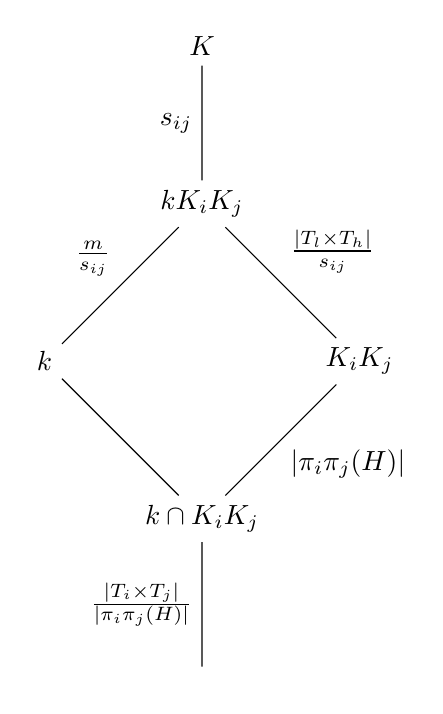
\begin{tikzpicture}
  \node (a) at (0,4)  {$K$};
  \node (b) at (0,2)  {$kK_iK_j$};
  \node (c) at (-2,0)  {$k$};
  \node (d) at (2,0)  {$K_iK_j$};
  \node (e) at (0,-2)  {$k\cap K_iK_j$};
  \node (f) at (0,-4)  {$\Q$};
  \draw   (a) -- node [left]{$s_{ij}$} (b) -- node [above left]{$\frac{m}{s_{ij}}$} (c) -- (e) -- node [below right]{$|\pi_i\pi_j(H)|$} (d) -- node [above right]{$\frac{|T_l\times T_h|}{s_{ij}}$} (b)
  (e) -- node [left]{$\frac{|T_i\times T_j|}{|\pi_i\pi_j(H)|}$} (f);
\end{tikzpicture}
%\vspace{3\baselineskip}
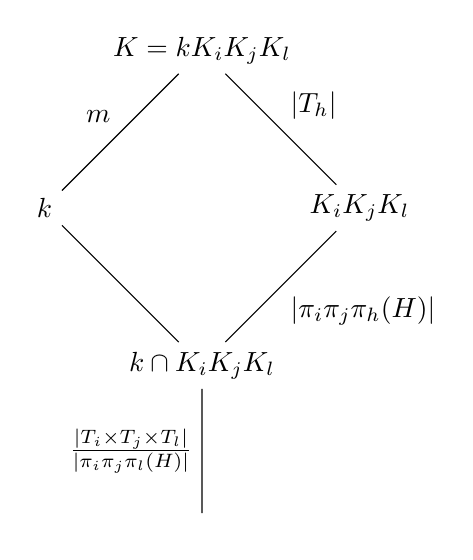
\begin{tikzpicture}
  \node (a) at (0,2)  {$K=kK_iK_jK_l$};
  \node (c) at (-2,0)  {$k$};
  \node (d) at (2,0)  {$K_iK_jK_l$};
  \node (e) at (0,-2)  {$k\cap K_iK_jK_l$};
  \node (f) at (0,-4)  {$\Q$};
  \draw   (a) -- node [above left]{$m$} (c) -- (e) -- node [below right ]{$|\pi_i\pi_j\pi_h(H)|$} (d) -- node [above right]{$|T_h|$} (a)
  (e) -- node [left]{$\frac{|T_i\times T_j\times T_l|}{|\pi_i\pi_j\pi_l(H)|}$} (f);
\end{tikzpicture}
\end{center}

\begin{rem}\label{remAN}
Note that Proposition \ref{degrees} implies that $a_in_i\neq 1$, otherwise $T_i$ would be trivial and $p_i$ wouldn't ramify in $k$.
\end{rem}

\begin{cor}\label{compcap}
We have $$[k\cap K_iK_j:\Q]=a_ia_j\frac{m}{r_ir_j}s_{ij},$$ $$[k\cap K_iK_jK_l:\Q]=a_ia_ja_l\frac{m^2}{r_ir_jr_l}$$ and $$[k:\Q]=a_1a_2a_3a_4\frac{m^3}{r_1r_2r_3r_4}.$$
\end{cor}
\begin{proof}
This follows from the computations
$$[k\cap K_iK_j:\Q]=\frac{[K_iK_j:\Q]}{[K_iK_j:k\cap K_iK_j]}=\frac{|T_i|\cdot|T_j|}{m/s_{ij}}=a_ia_j\frac{m}{r_ir_j}s_{ij},$$
$$[k\cap K_iK_jK_l:\Q]=\frac{[K_iK_jK_l:\Q]}{[K_iK_jK_l:k\cap K_iK_jK_l]}=\frac{|T_i|\cdot|T_j|\cdot|T_l|}{m}=a_ia_ja_l\frac{m^2}{r_ir_jr_l}$$
and
\begin{equation*}
\begin{split}
[k:\Q]&=\frac{[K:\Q]}{[K:k]}=\frac{|T_1|\cdot|T_2|\cdot|T_3|\cdot|T_4|}{m}=
a_1a_2a_3a_4\frac{m^3}{r_1r_2r_3r_4}.
%[k:\Q]&=[k\cap K_i:\Q]\cdot [k:k\cap K_i]=a_i\cdot [kK_i:K_i]=a_i\frac{[K:K_i]}{[K:kK_i]}\\
%&=a_i\frac{|T_j|\cdot|T_l|\cdot|T_h|}{r_i}=
%a_1a_2a_3a_4\frac{m^3}{r_1r_2r_3r_4}.
\end{split}
\end{equation*}

\end{proof}
\begin{lemma}\label{coprime}
We have 
$$s_{ij}=\gcd(r_i,r_j),$$ $$\gcd(r_i,r_j,r_l)=1,$$ $$\lcm\left(n_i,n_j,n_l\right)=m$$ and $$s_{ij}\frac{m}{r_ir_j}=\gcd(n_i,n_j).$$
\end{lemma}
\begin{proof}
It follows from Proposition \ref{degrees} that $s_{ij}\mid r_i, s_{ij}\mid r_j$ and $$|\pi_i(H)|=n_i, \quad |\pi_i\pi_j(H)|=\frac{m}{s_{ij}} \text{ and } |\pi_i\pi_j\pi_l(H)|=m.$$ The cyclicity of $H$ then implies
$$\frac{m}{s_{ij}}=|\pi_i\pi_j(H)|=|\langle\pi_i\pi_j(\tau)\rangle|=|\langle\pi_i(\tau)\pi_j(\tau)\rangle|=\lcm\left(n_i,n_j\right),$$
because $\langle\pi_i(\tau)\rangle=\pi_i(H)$ and any power of the product $\pi_i(\tau)\pi_j(\tau)$ is trivial if and only if the same power of both its factors is (since $G$ is the direct product of the $T_i$'s). 
%the elements $\pi_i(H),\pi_j(H)$ have different non-zero coordinates in $G$.
Now for any common divisor $t$ of $r_i,r_j$, we have $$\frac{m}{s_{ij}}= \lcm\left(n_i,n_j\right)=\lcm\left(\frac{m}{r_i},\frac{m}{r_j}\right) \mid \frac{m}{t},$$ which implies $t\mid s_{ij}$. Hence $s_{ij}=\gcd(r_i,r_j)$.

Similarly, we can compute
$$m=|\pi_i\pi_j\pi_l(H)|=|\langle\pi_i\pi_j\pi_l(\tau)\rangle|=|\langle\pi_i(\tau)\pi_j(\tau)\pi_l(\tau)\rangle|=\lcm(n_i,n_j,n_l).$$ In addition, if $t$ is any positive common divisor of $r_i,r_j,r_l$, we have $$m=\lcm(n_i,n_j,n_l)=\lcm\left(\frac{m}{r_i},\frac{m}{r_j},\frac{m}{r_l}\right) \mid \frac{m}{t},$$ which implies $t=1$, hence $\gcd(r_i,r_j,r_l)=1$.

Finally, using the first result, we have $$s_{ij}\frac{m}{r_ir_j}=\frac{m}{r_ir_j/s_{ij}}=\frac{m}{\lcm(r_i,r_j)},$$ which clearly divides both $\frac{m}{r_i}=n_i$ and $\frac{m}{r_j}=n_j$. Moreover, if $t$ is any common divisor of $n_i=\frac{m}{r_i}$ and $n_j=\frac{m}{r_j}$, then both $r_it$ and $r_jt$ divide $m$, hence $t\cdot\lcm(r_i,r_j)=\lcm(r_it,r_jt)\mid m$. Thus $t\mid \frac{m}{\lcm(r_i,r_j)}$ and we are done.
\end{proof}

\begin{rem}
If $k$ is fixed, we have shown in Lemmas \ref{degrees} and \ref{coprime} and Remark \ref{remAN} that $$r_i\mid m, \gcd(r_i,r_j,r_l)=1, a_in_i\neq 1.$$
Conversely, using the theory of Dirichlet characters, it can be shown that for any choice of positive integers
$m,a_1,a_2,a_3,a_4,r_1,r_2,r_3,r_4$ satisfying
$$r_i\mid m, \gcd(r_i,r_j,r_l)=1, a_in_i\neq 1,$$
there exist infinitely many real abelian fields $k$ ramified at exactly four primes satisfying the assumptions on page \pageref{assum} (in particular, the family of fields we are studying is nonempty). The proof of this is analogous to the proof of a similar statement in \citep{Azar} and we omit it.
\end{rem}

\begin{prop}\label{gal}
We have 
\begin{equation*}
\begin{split}
\Gal(k/\Qbb)\cong
 \{\restr{\sigma_1^{x_1}\sigma_2^{x_2}\sigma_3^{x_3}\sigma_4^{x_4}}{k};~ & 0\leq x_1<a_1\frac{m}{r_1}, 0\leq x_2<a_2\frac{m}{r_2s_{34}}, \\ & 0\leq x_3<a_3\frac{m}{r_3r_4}s_{34},0\leq x_4<a_4\},
\end{split}
\end{equation*}
where each automorphism of $k$ determines the quadruple $(x_1,x_2,x_3,x_4)$ uniquely.
\end{prop}
\begin{proof}
First note that by Lemma \ref{coprime}, we have $$a_3\frac{m}{r_3r_4}s_{34}=a_3\gcd(n_3,n_4)\in\Nbb$$ and $$a_2\frac{m}{r_2s_{34}}\in\Nbb$$ (this follows from $r_2\mid m$, $s_{34}\mid m$ and $\gcd(r_2,s_{34})=\gcd(r_2,r_3,r_4)=1$), so the expressions make sense. By Corollary \ref{compcap}, the set on the right hand side has at most $|\Gal(k/\Qbb)|$ elements. Now let $\rho$ be any automorphism of $k$. %If we can show that $\rho$ determines the quadruple $(x_1,x_2,x_3,x_4)$ belonging to the set on the right hand side uniquely, it will follow that the cardinalities agree and we will be done.
If we can show that $\rho$ can be written as $$\rho=\sigma_1^{x_1}\sigma_2^{x_2}\sigma_3^{x_3}\sigma_4^{x_4}\mid_k$$ for a unique quadruple $(x_1,x_2,x_3,x_4)$ satisfying $$0\leq x_1<a_1\frac{m}{r_1}, 0\leq x_2<a_2\frac{m}{r_2s_{34}}, 0\leq x_3<a_3\frac{m}{r_3r_4}s_{34},0\leq x_4<a_4\},$$ it will follow that the cardinalities agree and we will be done.

\begin{center}
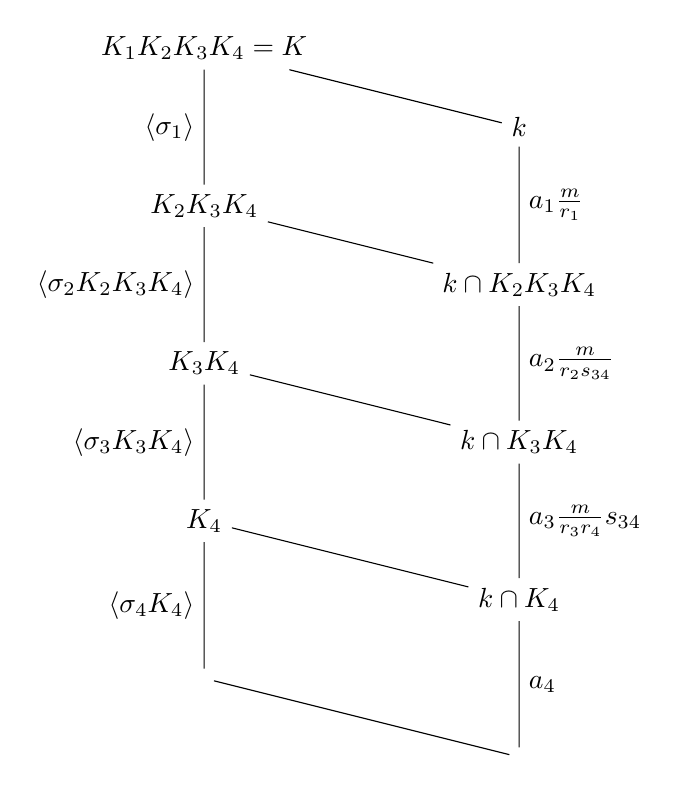
\begin{tikzpicture}
  \node (a) at (0,4)  {$K_1K_2K_3K_4=K$};
  \node (b) at (4,3)  {$k$};
  \node (c) at (0,2)  {$K_2K_3K_4$};
  \node (d) at (4,1)  {$k\cap K_2K_3K_4$};
  \node (e) at (0,0)  {$K_3K_4$};
  \node (f) at (4,-1)  {$k\cap K_3K_4$};
  \node (g) at (0,-2) {$K_4$};
  \node (h) at (4,-3)  {$k\cap K_4$};
  \node (i) at (0,-4) {$\Q$};
  \node (j) at (4,-5)  {$\Q$};
  \draw  (a) -- node [midway,left]{$\langle \sigma_1\rangle$} (c) -- node [midway,left]{$\langle \restr{\sigma_2}{K_2K_3K_4}\rangle$} (e) -- node [midway,left]{$\langle \restr{\sigma_3}{K_3K_4}\rangle$} (g) -- node [midway,left]{$\langle \restr{\sigma_4}{K_4}\rangle$} (i) -- (j) -- node [midway,right]{$a_4$} (h) -- node [midway,right]{$a_3\frac{m}{r_3r_4}s_{34}$} (f) -- node [midway,right]{$a_2\frac{m}{r_2s_{34}}$} (d) -- node [midway,right]{$a_1\frac{m}{r_1}$} (b) -- (a) 
  (c) -- (d)
  (e) -- (f)
  (g) -- (h);
\end{tikzpicture}
\end{center}

Since $\Gal(k\cap K_4/\Q)$ is a cyclic group of order $a_4$ (by Lemma \ref{degrees}) generated by $\restr{\sigma_4}{k\cap K_4}$ (as a quotient of $\Gal(K_4/\Q)=\langle \restr{\sigma_4}{K_4}\rangle$), there must exist a unique $x_4\in \Z$, $0\leq x_4<a_4$ such that $\rho$ and $\sigma_4^{x_4}$ have the same restrictions to $k\cap K_4$. Therefore $\rho\restr{\sigma_4^{-x_4}}{k}\in \Gal(k/k\cap K_4)$. 

Next, $\Gal(k\cap K_3K_4/k\cap K_4)$ is a cyclic group of order $\frac{[k\cap K_3K_4:\Q]}{[k\cap K_4:\Q]}=a_3\frac{m}{r_3r_4}s_{34}$ (by Corollary \ref{compcap}) generated by $\restr{\sigma_3}{k\cap K_3K_4}$ (as it is isomorphic by restriction to $$\Gal((k\cap K_3K_4)K_4 / K_4),$$ which is a quotient of $\Gal(K_3K_4/K_4)=\langle \restr{\sigma_3}{K_3K_4}\rangle$), so there must exist a unique $x_3\in \Z$ with $0\leq x_3<a_3\frac{m}{r_3r_4}s_{34}$ such that $\rho \restr{\sigma_4^{-x_4}}{k}$ and $\sigma_3^{x_3}$ have the same restriction to $k\cap K_3K_4$. Therefore $\restr{\rho\sigma_3^{-x_3}\sigma_4^{-x_4}}{k}\in \Gal(k/k\cap K_3K_4)$.

Following the pattern, $\Gal(k\cap K_2K_3K_4/k\cap K_3K_4)$ is a cyclic group of order 
$$\frac{[k\cap K_2K_3K_4:\Q]}{[k\cap K_3K_4:\Q]}=a_2\frac{m}{r_2s_{34}}$$ (by Corollary \ref{compcap}) generated by $\restr{\sigma_2}{k\cap K_2K_3K_4}$ (as it is isomorphic by restriction to $$\Gal((k\cap K_2K_3K_4)K_3K_4 / K_3K_4),$$ which is a quotient of $$\Gal(K_2K_3K_4/K_3K_4)=\langle \restr{\sigma_2}{K_2K_3K_4}\rangle),$$ so there must exist a unique $x_2\in \Z$, $0\leq x_2<a_2\frac{m}{r_2s_{34}}$ such that $\rho\restr{\sigma_3^{-x_3}\sigma_4^{-x_4}}{k}$ and $\sigma_2^{x_2}$ have the same restriction to $k\cap K_2K_3K_4$. Therefore $\restr{\rho\sigma_2^{-x_2}\sigma_3^{-x_3}\sigma_4^{-x_4}}{k}\in \Gal(k/k\cap K_2K_3K_4)$.

Finally, we have $$\Gal(k/k\cap K_2K_3K_4)\cong \Gal(kK_2K_3K_4/K_2K_3K_4)=\Gal(K_1K_2K_3K_4/K_2K_3K_4)=\langle\sigma_1\rangle$$
(using Lemma \ref{genus}), where the isomorphism is given by restriction. Since the order of $\sigma_1$ is $a_1\frac{m}{r_1}$, it follows that there must exist a unique $x_1\in \Z$, $0\leq x_1<a_1\frac{m}{r_1}$ such that $\rho\restr{\sigma_2^{-x_2}\sigma_3^{-x_3}\sigma_4^{-x_4}}{k}$ and $\sigma_1^{x_1}$ have the same restriction to $k$. Thus $\rho=\restr{\sigma_1^{x_1}\sigma_2^{x_2}\sigma_3^{x_3}\sigma_4^{x_4}}{k}$ and the proof is finished.

\end{proof}